\documentclass[conference]{IEEEtran}
\IEEEoverridecommandlockouts
\usepackage{amsmath,amssymb,amsthm,mathtools}
\usepackage{graphicx}
\usepackage{booktabs}
\usepackage{multirow}
\usepackage{xcolor}
\usepackage{algorithm}
\usepackage{algpseudocode}
\usepackage[hidelinks]{hyperref}
\usepackage{cleveref}

\newtheorem{theorem}{Theorem}
\newtheorem{proposition}{Proposition}
\newtheorem{lemma}{Lemma}
\newtheorem{corollary}{Corollary}
\theoremstyle{definition}
\newtheorem{definition}{Definition}
\newtheorem{remark}{Remark}
\newtheorem{example}{Example}

\newcommand{\sys}{\textup{\textsc{Ville}}}
\newcommand{\E}{\mathbb{E}}
\newcommand{\Prb}{\mathbb{P}}
\newcommand{\F}{\mathcal{F}}
\newcommand{\todo}[1]{\textcolor{red}{[#1]}}
% generated by make_macros.py; do not edit
\newcommand{\numAMZLBETVSWSR}{1.3}
\newcommand{\numAMZLBOUNDEFF}{1.3}
\newcommand{\numAMZLPROXYEFF}{1.3}
\newcommand{\numAMZLRBET}{1.3}
\newcommand{\numAMZLRBSP}{2.6}
\newcommand{\numAMZLRCLT}{1.00}
\newcommand{\numAMZLRCLTP}{0.74}
\newcommand{\numAMZLRHS}{2.0}
\newcommand{\numAMZLRWSR}{1.7}
\newcommand{\numAMZSBETVSWSR}{1.8}
\newcommand{\numAMZSBOUNDEFF}{1.6}
\newcommand{\numAMZSPROXYEFF}{1.8}
\newcommand{\numAMZSRBET}{1.6}
\newcommand{\numAMZSRBSP}{3.7}
\newcommand{\numAMZSRCLT}{1.10}
\newcommand{\numAMZSRCLTP}{0.70}
\newcommand{\numAMZSRHS}{3.7}
\newcommand{\numAMZSRWSR}{2.9}
\newcommand{\numAXAREARHS}{1.8}
\newcommand{\numAXAREARWSR}{1.9}
\newcommand{\numAXBETVSWSR}{1.7}
\newcommand{\numAXBOUNDEFF}{1.6}
\newcommand{\numAXPROXYEFF}{1.6}
\newcommand{\numAXRBET}{1.5}
\newcommand{\numAXRBSP}{3.8}
\newcommand{\numAXRCLT}{1.03}
\newcommand{\numAXRCLTP}{0.72}
\newcommand{\numAXRHS}{2.2}
\newcommand{\numAXRWSR}{2.5}
\newcommand{\numAXRWSRMAX}{4.5}
\newcommand{\numAXYEARRHS}{2.9}
\newcommand{\numAXYEARRWSR}{3.4}
\newcommand{\numBETVSWSR}{1.6}
\newcommand{\numBINA}{1.6}
\newcommand{\numBINAN}{27}
\newcommand{\numBINB}{2.1}
\newcommand{\numBINBN}{30}
\newcommand{\numBINC}{4.8}
\newcommand{\numBINCN}{18}
\newcommand{\numBOUNDEFF}{1.5}
\newcommand{\numCVMAX}{30}
\newcommand{\numCVMED}{9}
\newcommand{\numCVSEMAX}{5.4}
\newcommand{\numLLMBETVSWSR}{1.4}
\newcommand{\numLLMBOUNDEFF}{1.4}
\newcommand{\numLLMPROXYEFF}{1.4}
\newcommand{\numLLMRBET}{1.4}
\newcommand{\numLLMRBSP}{2.9}
\newcommand{\numLLMRCLT}{1.01}
\newcommand{\numLLMRCLTP}{0.73}
\newcommand{\numLLMRHS}{2.1}
\newcommand{\numLLMRWSR}{1.9}
\newcommand{\numNCLTERR}{5}
\newcommand{\numNCLTERRQ}{2}
\newcommand{\numNCLTPERR}{3}
\newcommand{\numNCLTPERRQ}{2}
\newcommand{\numNCV}{75}
\newcommand{\numNEXEC}{2{,}250}
\newcommand{\numNLEBSP}{75}
\newcommand{\numNLEHS}{74}
\newcommand{\numNLEWSR}{75}
\newcommand{\numNPROXYQ}{75}
\newcommand{\numNPROXYWRONG}{31}
\newcommand{\numNQ}{75}
\newcommand{\numNQA}{12}
\newcommand{\numNQL}{27}
\newcommand{\numNQLLM}{39}
\newcommand{\numNQS}{36}
\newcommand{\numPROXYEFF}{1.6}
\newcommand{\numPROXYSAVEMAX}{82}
\newcommand{\numPROXYSAVEMIN}{45}
\newcommand{\numRBET}{1.5}
\newcommand{\numRBSP}{3.3}
\newcommand{\numRCLT}{1.05}
\newcommand{\numRCLTP}{0.72}
\newcommand{\numRCLTPINV}{1.4}
\newcommand{\numRHOGS}{0.71}
\newcommand{\numRHS}{2.8}
\newcommand{\numRWSR}{2.3}
\newcommand{\numRWSRMAX}{8.2}

% generated from completed live measurements by make_online_table.py
\newcommand{\numLiveHavingMin}{2.5}
\newcommand{\numLiveHavingMax}{16.0}
\newcommand{\numLiveMaxOverhead}{0.2}
\newcommand{\numLiveN}{32{,}000}


\begin{document}

\title{\sys: Certified Decision Queries over LLM-Evaluated Data with Proxy-Rectified E-Processes}

\author{\IEEEauthorblockN{Yanbo Bian\textsuperscript{*}}
\IEEEauthorblockA{Weihai International College\\
Beijing Jiaotong University\\
Weihai, China\\
24722081@bjtu.edu.cn\\
\href{https://orcid.org/0009-0003-0014-8435}{ORCID 0009-0003-0014-8435}}
\and
\IEEEauthorblockN{Zhihai Wang\textsuperscript{*}}
\IEEEauthorblockA{Beijing Jiaotong University\\
Beijing, China\\
zhhwang@bjtu.edu.cn\\
\href{https://orcid.org/0009-0000-4036-9396}{ORCID 0009-0000-4036-9396}}
\thanks{\textsuperscript{*}Corresponding authors.}}
\hypersetup{pdfauthor={Yanbo Bian and Zhihai Wang}}

\maketitle

\begin{abstract}
LLM-powered analytics answers group-level decision queries, such as HAVING thresholds, rankings, and top-$k$ selections over LLM-judged attributes, with one model call per tuple.
Sampling reduces this cost, but a sampled decision needs a guarantee that survives continuous monitoring.
Confidence sequences can stop once a threshold claim is settled, but they bound each group's mean on its own and ignore the proxy scores the system already holds; proxy-based estimators use those scores but certify estimates at a fixed sample size, not decisions under continuous monitoring.
We present \sys{}, a decision layer that compiles HAVING, ORDER BY, and Top-$k$ queries into a handful of boundary hypotheses and tests each with a betting e-process, which stays valid at any stopping time by Ville's inequality.
It bets on proxy-rectified values, which keep every group mean exact for any proxy while removing the variance that the proxy explains.
Finite-population and paired forms of the tests handle sampling without replacement and groups of very different sizes.
We prove that \sys{} returns an incorrect answer with probability at most $\alpha$ under any stopping rule and any proxy.
On \numNQ{} queries over three datasets, including 122 thousand reviews and 309 thousand paper abstracts judged by a real LLM, \sys{} returned no incorrect answer in \numNEXEC{} executions.
It used \numRWSR$\times$ fewer LLM calls than Evergreen-style confidence sequences (up to \numRWSRMAX$\times$ on large groups) and \numRHS--\numRBSP$\times$ fewer than IFOCUS- and BlazeIt-style bounds, and about as many as uncertified normal-approximation stopping, which returned wrong answers in up to 13\% of a query's executions.
With two LLMs in the loop, latency followed the number of calls, and HAVING queries ran \numLiveHavingMin$\times$ and \numLiveHavingMax$\times$ faster than full evaluation.
\end{abstract}

\section{Introduction}
\label{sec:intro}

Large language models have turned free text into a queryable attribute.
Systems with semantic operators let an analyst filter, rank, and aggregate records by natural-language criteria that an LLM evaluates tuple by tuple~\cite{lotus,docetl,uqe,thalamusdb}.
Many of the questions asked this way are \emph{decisions over groups}.
A product manager asks which product lines have more than 20\% of reviews reporting a defect (a HAVING query).
A support lead ranks stores by LLM-judged service quality (ORDER BY).
A dashboard shows the five categories with the most negative reviews (Top-$k$).
Evaluating such a query exactly issues one LLM call per tuple.
For the 6.8 million reviews in our evaluation, that is 6.8 million calls and about 860 million input tokens with our prompts, for a single attribute and before the first answer is shown.

Sampling is the natural remedy, and decision queries are where a sampled answer most needs a guarantee.
An estimate that is off by a percentage point is harmless, but a group placed on the wrong side of a threshold or a swapped pair in a ranking is a wrong answer, and nothing in the sample reveals it.
The common practice of sampling until normal-approximation intervals separate provides no such guarantee: the intervals are valid at one pre-planned sample size, and checking them after every batch, as analysts and agents do, inflates the error rate by an amount that depends on the data~\cite{johari2022,ramdas2023savi}.
Certified alternatives exist, but they are expensive.
Range-based bounds with a union bound over checks, as in IFOCUS~\cite{ifocus}, pay for the worst case.
Evergreen uses confidence sequences to stop as soon as a threshold claim is confirmed or refuted, including under sampling without replacement~\cite{evergreen,wsr2024betting}.
A confidence sequence, however, bounds each group's mean on its own: comparing two groups requires both intervals to clear the gap, and Evergreen's estimates do not use the proxy scores that LLM-powered systems already compute.

Proxies are the standard lever for expensive predicates.
BlazeIt and ABae use them to reduce the variance of aggregate estimates~\cite{blazeit,abae}, SUPG to select records with precision or recall targets~\cite{supg}, and LOTUS and BARGAIN to route tuples between cheap and expensive models~\cite{lotus,bargain}.
These methods certify estimates, selections, or tuple-level outputs, mostly at a fixed sample size.
A proxy cannot replace the LLM, however: in our evaluation, answers computed from proxy scores alone were wrong for \numNPROXYWRONG{} of \numNPROXYQ{} queries.
What remains open is how few LLM calls suffice to certify a group-level \emph{decision} when the answer is monitored continuously and a proxy of unknown quality is available.

We answer this question with \sys{}, a decision layer for HAVING, ORDER BY, and Top-$k$ queries over LLM-evaluated attributes.
\sys{} rests on three observations.
First, a decision depends on a few boundary hypotheses, such as ``the mean exceeds the threshold'' or ``group $i$ beats group $j$'', which let \sys{} adapt each bet to the gap relevant to that comparison.
Second, each boundary hypothesis can be tested by betting: the bettor's wealth is a nonnegative supermartingale under the null, and Ville's inequality~\cite{ville1939} bounds the error at every stopping time.
Third, the bets can be placed on proxy-rectified values $y-\beta(p-\bar p_g)$, which have exactly the group mean of the LLM judgments for any proxy, and far smaller variance when the proxy is informative.
\sys{} realizes these observations for sampling without replacement, pairs groups of very different sizes with an exactly unbiased per-draw statistic, and stops each group as soon as its decisions are certified.

This paper makes the following contributions.
\begin{itemize}
\item We define certified decision queries over LLM-evaluated attributes, with an indifference margin that makes certification possible before every tuple is judged (\Cref{sec:problem}).
\item We design proxy-rectified boundary e-processes for single groups and for pairs under sampling without replacement, and prove that \sys{} returns an incorrect answer with probability at most $\alpha$ under any stopping rule and any proxy (\Cref{sec:method}).
\item We compile HAVING, ORDER BY, and Top-$k$ queries into these tests with per-group adaptive stopping (\Cref{sec:processing}).
\item We evaluate \sys{} on \numNQ{} queries over three datasets, two of them judged by a real LLM. \sys{} never returned an incorrect answer, used \numRWSR$\times$ fewer LLM calls than Evergreen-style confidence sequences (up to \numRWSRMAX$\times$) and \numRHS--\numRBSP$\times$ fewer than IFOCUS- and BlazeIt-style bounds, and needed about as many calls as uncertified sampling, which erred in up to 13\% of executions. With two LLMs in the loop, latency followed the number of calls, and HAVING queries ran \numLiveHavingMin$\times$ and \numLiveHavingMax$\times$ faster than full evaluation (\Cref{sec:exp}).
\end{itemize}

\section{Problem Setting}
\label{sec:problem}

\begin{figure*}[t]
\centering
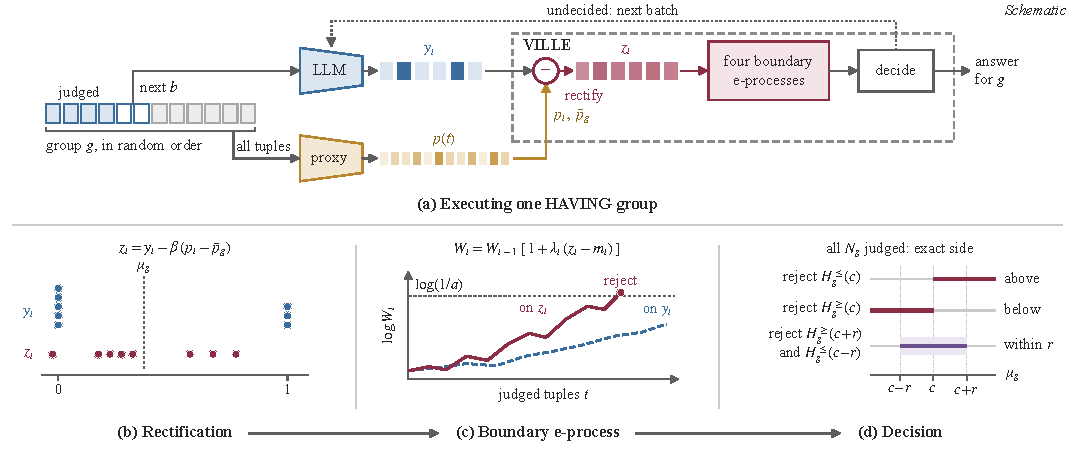
\includegraphics[width=\textwidth]{figures/overview_mechanism.pdf}
\caption{\sys{} executing one HAVING group. (a) In one random order, the LLM judges the next $b$ tuples, the proxy scores all tuples once, and \sys{} rectifies the judgments and updates four boundary e-processes until a decision is certified. (b) Rectification keeps the group mean $\mu_g$ for any proxy, and an informative proxy pulls 0/1 judgments toward it (eight tuples, $\beta=1$). (c) Each e-process bets against the remaining-population null mean $m_t$ (\Cref{eq:mt}) and rejects at wealth $1/a$, $a=\alpha/(2K)$; betting on $y_t$ (dashed) is slower. (d) Rejections that certify each answer; an exhausted group is decided exactly.}
\label{fig:overview}
\end{figure*}


\subsection{Decision queries over an expensive attribute}

We consider a relation $R$ whose tuples are partitioned into $K$ groups by a grouping key, for example the product, brand, category, or year of a review.
Group $g$ contains $N_g$ tuples.
The sizes $N_g$ are known, because counting tuples per group only reads the grouping column.
Each tuple $t$ has an \emph{expensive attribute} $y(t)\in[y_{\min},y_{\max}]$ that is obtained by one call to a large language model (LLM).
For a semantic predicate such as ``does this review report a defective product?'', $y(t)\in\{0,1\}$.
For a semantic score such as ``how positive is this review, from 1 to 5?'', $y(t)\in[1,5]$.
We treat the LLM as a deterministic function of the tuple, as with greedy decoding and a cache, so each tuple is judged at most once.
The query targets the group means
\begin{equation}
\mu_g=\frac{1}{N_g}\sum_{t\in g} y(t), \qquad g=1,\dots,K .
\end{equation}
\texttt{AVG} over a score and the fraction of tuples satisfying a predicate are both of this form.
\texttt{COUNT} and \texttt{SUM} equal $N_g\mu_g$, so decisions on them reduce to decisions on $\mu_g$ with a rescaled threshold.

The system also has a \emph{proxy} $p(t)\in[y_{\min},y_{\max}]$ for every tuple, for example a small classifier on n-grams or embeddings.
Proxies are orders of magnitude cheaper than LLM calls and are routinely used to optimize queries with expensive model predicates~\cite{blazeit,supg,abae,lotus,bargain}.
We make no assumption on proxy quality: a poor proxy may cost efficiency, but it must never cost correctness.

We study three \emph{decision queries}, whose answers are discrete:
\begin{itemize}
\item \textbf{HAVING}: return the groups with $\mu_g>c$ for a threshold $c$.
\item \textbf{ORDER BY}: return the groups ranked by $\mu_g$.
\item \textbf{Top-$k$}: return the $k$ groups with the largest $\mu_g$ (\texttt{ORDER BY \dots\ LIMIT} $k$).
\end{itemize}
These queries are the backbone of dashboards and of LLM-generated reports (``which product lines have more than 20\% defect complaints?'', ``rank the stores by service quality'', ``the five categories with the most negative reviews'').
They are also the queries that a sampling-based answer can get \emph{wrong}: an estimate that is off by one percentage point is harmless, whereas a swapped pair in a ranking or a group on the wrong side of a threshold is a wrong answer.

\subsection{Correctness with an indifference margin}

Exact decisions cannot be certified from samples when two means coincide or a mean sits on the threshold.
We therefore adopt an indifference margin $r>0$, a standard device in sequential selection~\cite{bechhofer1954,lucb}.

\begin{definition}[$r$-correct answers]
\label{def:rcorrect}
A HAVING answer $A\subseteq[K]$ is $r$-correct if every group with $\mu_g\ge c+r$ is in $A$ and no group with $\mu_g\le c-r$ is in $A$.
A ranking is $r$-correct if group $i$ precedes group $j$ whenever $\mu_i\ge \mu_j+r$.
A Top-$k$ answer $S$ with $|S|=k$ is $r$-correct if $\min_{i\in S}\mu_i\ge \mu_{(k)}-r$, where $\mu_{(k)}$ is the $k$-th largest group mean.
\end{definition}

Groups or pairs inside the margin may be reported either way.
The margin is part of the query, for example $r=5\%$ of the overall mean.
It permits early termination near a boundary through an ``indifferent'' certificate. Every finite group also has an exact fallback when all its tuples have been judged.

\subsection{Certified answers and cost}

A system answers a decision query by repeatedly sending batches of sampled tuples to the LLM, updating its statistics, and deciding when to stop.
Analysts and LLM agents also inspect intermediate answers and stop when the answer looks stable.
Both behaviours are forms of \emph{continuous monitoring}.
A fixed-sample confidence interval does not survive them: its coverage holds only at one pre-specified sample size~\cite{ramdas2023savi,johari2022}.

\begin{definition}[Certified decision query]
\label{def:certified}
An algorithm certifies a decision query at level $\alpha$ if, for every data instance, every proxy, and every (possibly data-dependent) stopping time, the probability that it reports an answer that is not $r$-correct is at most $\alpha$.
\end{definition}

The cost of an algorithm is the number of LLM calls it issues, $C=\sum_g n_g$, where $n_g\le N_g$ is the number of tuples of group $g$ that were judged.
We report $C/\sum_g N_g$, the fraction of the full evaluation that was needed.
Proxy scores are computed once for all tuples and their cost is amortized; we report it separately.
The goal is to certify every decision query at level $\alpha$ with as few LLM calls as possible.

\section{Proxy-Rectified Boundary E-Processes}
\label{sec:method}

\begin{figure*}[t]
\centering
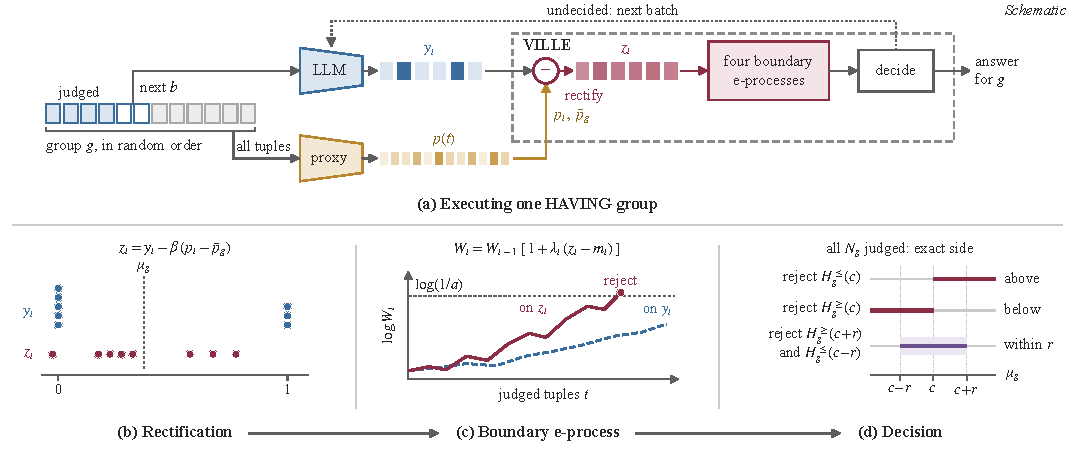
\includegraphics[width=\textwidth]{figures/overview_mechanism.pdf}
\caption{\sys{} executing one HAVING group. (a) In one random order, the LLM judges the next $b$ tuples, the proxy scores all tuples once, and \sys{} rectifies the judgments and updates four boundary e-processes until a decision is certified. (b) Rectification keeps the group mean $\mu_g$ for any proxy, and an informative proxy pulls 0/1 judgments toward it (eight tuples, $\beta=1$). (c) Each e-process bets against the remaining-population null mean $m_t$ (\Cref{eq:mt}) and rejects at wealth $1/a$, $a=\alpha/(2K)$; betting on $y_t$ (dashed) is slower. (d) Rejections that certify each answer; an exhausted group is decided exactly.}
\label{fig:overview}
\end{figure*}


\sys{} rests on three ideas.
First, it never estimates a group mean for its own sake; it tests only the few hypotheses that decide the answer (\Cref{sec:boundary}).
Second, each hypothesis is tested by a betting e-process, which stays valid under continuous monitoring and adaptive sampling (\Cref{sec:betting}).
Third, the e-process bets on proxy-rectified values, which keep the group mean intact while removing the variance that the proxy explains (\Cref{sec:rectify}).
\Cref{fig:overview} shows how the three fit together for one HAVING group.
\Cref{sec:wor,sec:pair} give the without-replacement forms for single groups and for pairs, and \Cref{sec:guarantee} states the guarantees.

\subsection{From decisions to boundary hypotheses}
\label{sec:boundary}

A decision query depends on the data only through a few comparisons.
For HAVING, group $g$ is answered by the outcome of four one-sided hypotheses:
\begin{equation}
\begin{aligned}
&H^{\le}_{g}(c):\mu_g\le c, && H^{\ge}_{g}(c):\mu_g\ge c,\\
&H^{\ge}_{g}(c+r):\mu_g\ge c+r, && H^{\le}_{g}(c-r):\mu_g\le c-r.
\end{aligned}
\end{equation}
Rejecting $H^{\le}_g(c)$ certifies ``above'', rejecting $H^{\ge}_g(c)$ certifies ``below'', and rejecting both $H^{\ge}_g(c+r)$ and $H^{\le}_g(c-r)$ certifies $|\mu_g-c|<r$, in which case either answer is $r$-correct.
For a pair of groups $(i,j)$, the same four hypotheses are posed on the difference $\mu_i-\mu_j$ with boundaries $0$ and $\pm r$.
ORDER BY and Top-$k$ are assembled from pair outcomes (\Cref{sec:processing}).

This formulation exposes the null value and direction relevant to each decision.
\sys{} uses them to choose a gap-adaptive bet for each boundary (\Cref{eq:lambda}) and to test group differences directly (\Cref{sec:pair}).
Both our tests and the confidence-sequence baselines stop when a side or an indifference decision is certified. The experimental comparison measures the combined effects of the betting rule and the paired construction.

\subsection{Testing by betting}
\label{sec:betting}

Consider a stream $z_1,z_2,\dots$ in $[\ell,h]$ and a null hypothesis that bounds the conditional mean of each observation by $m_t$, i.e., $\E[z_t\mid\F_{t-1}]\le m_t$.
A gambler starts with wealth $W_0=1$ and, before seeing $z_t$, stakes a fraction $\lambda_t\ge 0$ chosen from the past:
\begin{equation}
W_t=W_{t-1}\bigl(1+\lambda_t(z_t-m_t)\bigr).
\label{eq:wealth}
\end{equation}
If $\lambda_t\le\kappa/(m_t-\ell)$ for a constant $\kappa<1$, the wealth stays positive.
Under the null, $\E[W_t\mid\F_{t-1}]\le W_{t-1}$, so $(W_t)$ is a nonnegative supermartingale, or \emph{e-process}~\cite{ramdas2023savi,shafer2021}.
By Ville's inequality~\cite{ville1939},
\begin{equation}
\Prb\bigl(\exists t:\ W_t\ge 1/a\bigr)\le a .
\label{eq:ville}
\end{equation}
Rejecting the null as soon as the wealth reaches $1/a$ therefore has type-I error at most $a$, no matter how often the wealth is inspected, when sampling stops, or how the system decides which group to sample next.
This is exactly the protection that continuous monitoring requires, and it is what fixed-sample intervals lack.

The betting fraction determines power, and we use an approximately growth-rate-optimal fraction in the spirit of aGRAPA~\cite{wsr2024betting}:
\begin{equation}
\lambda_t=\min\Bigl\{\max\Bigl\{\frac{\hat\gamma_{t}}{\hat\sigma^2_{t}+\hat\gamma_{t}^2},\,0\Bigr\},\ \frac{\kappa}{m_t-\ell}\Bigr\},\qquad \kappa=\tfrac12,
\label{eq:lambda}
\end{equation}
where $\hat\gamma_t$ is the predicted excess of $\E[z_t\mid\F_{t-1}]$ over $m_t$ and $\hat\sigma^2_t$ is a running variance estimate, both computed from $z_1,\dots,z_{t-1}$ with one pseudo-observation on the null boundary.
Any predictable choice keeps the guarantee; this one makes the log-wealth grow at roughly $\gamma^2/(2\sigma^2)$ per call when the true excess is $\gamma$ and the variance is $\sigma^2$.
A test therefore rejects after about
\begin{equation}
n\approx\frac{2\sigma^2\log(1/a)}{\gamma^2}
\label{eq:cost}
\end{equation}
calls.
\Cref{eq:cost} explains where \sys{} saves: decisions pay $1/\gamma^2$ only for groups near a boundary, and the variance $\sigma^2$ is the target of the next step.

\subsection{Proxy rectification}
\label{sec:rectify}

Let $\bar p_g=\frac1{N_g}\sum_{t\in g}p(t)$ be the mean proxy score of group $g$, which is computed exactly because proxies are cheap.
For a weight $\beta\in[0,1]$, define the \emph{rectified value}
\begin{equation}
z(t)=y(t)-\beta\bigl(p(t)-\bar p_g\bigr),\qquad t\in g .
\label{eq:rectify}
\end{equation}

\begin{lemma}[Rectification preserves the group mean]
\label{lem:unbiased}
For every proxy and every $\beta$, $\sum_{t\in g}z(t)=N_g\mu_g$.
\end{lemma}
\begin{proof}
$\sum_{t\in g}z(t)=\sum_{t\in g}y(t)-\beta\bigl(\sum_{t\in g}p(t)-N_g\bar p_g\bigr)=N_g\mu_g$.
\end{proof}

The population of rectified values has exactly the group mean that the query asks about, so every test of \Cref{sec:boundary} can be run on $z$ instead of $y$.
Rectified values are the control-variate form that BlazeIt uses for estimation~\cite{blazeit} and the rectifier of prediction-powered inference~\cite{ppi,avppi,ppevalues}; \sys{} places them inside boundary tests under sampling without replacement.
Their variance is $\mathrm{Var}_g(y)-2\beta\,\mathrm{Cov}_g(y,p)+\beta^2\mathrm{Var}_g(p)$.
For $\mathrm{Var}_g(p)>0$, the population-optimal coefficient in $[0,1]$ is $\beta_g^\star=\min\{1,\max\{0,\mathrm{Cov}_g(y,p)/\mathrm{Var}_g(p)\}\}$.
When the unconstrained optimum lies in this interval, its variance is $(1-\rho_g^2)\mathrm{Var}_g(y)$, where $\rho_g$ is the correlation between the LLM judgment and the proxy.
At this ideal coefficient, \Cref{eq:cost} suggests roughly twofold and fivefold call savings at $\rho=0.71$ and $\rho=0.89$. Our implementation estimates a shared coefficient from an independent training set, and its variance follows the quadratic expression above.
A useless proxy gives $\rho=0$ and leaves the variance unchanged at $\beta=0$; even a misleading proxy only enlarges the variance.
Because \Cref{lem:unbiased} holds for every proxy, proxy quality affects cost and never validity.
We fix $\beta$ before the query from the small labeled set used to train the proxy; any data-independent $\beta$ is valid.

Rectification widens the range of the values: with $y,p\in[y_{\min},y_{\max}]$, the rectified values of group $g$ lie in $[\ell_g,h_g]=[y_{\min}-\beta(y_{\max}-\bar p_g),\ y_{\max}-\beta(y_{\min}-\bar p_g)]$, up to twice the original width.
Range-based bounds such as Hoeffding's pay for this growth in full.
The betting fraction in \Cref{eq:lambda} adapts to the variance and touches the range only through the cap, so \sys{} keeps most of the variance reduction.

\subsection{Sampling without replacement}
\label{sec:wor}

A tuple is judged at most once, so the tuples of a group are drawn without replacement: \sys{} draws a uniformly random permutation of group $g$ and judges its prefix.
Let $S_{t-1}=\sum_{s<t}z_s$ be the sum of the first $t-1$ rectified values.
Under without-replacement sampling,
\begin{equation}
\E[z_t\mid\F_{t-1}]=\frac{N_g\mu_g-S_{t-1}}{N_g-t+1}.
\end{equation}
Hence, under $H^{\le}_g(m)$, the conditional mean of the $t$-th draw is at most
\begin{equation}
m_t=\frac{N_g m-S_{t-1}}{N_g-t+1},
\label{eq:mt}
\end{equation}
which is the null value to plug into \Cref{eq:wealth}.

\begin{proposition}[One-sample test]
\label{prop:one}
Draw group $g$ without replacement and run \Cref{eq:wealth} on $z$ with $m_t$ from \Cref{eq:mt}, $\lambda_t$ predictable and $0\le\lambda_t\le\kappa/(m_t-\ell_g)$ with $\kappa<1$, $\lambda_t=0$ when $m_t\ge h_g$, and immediate rejection when $m_t<\ell_g$.
Then, under $H^{\le}_g(m)$, $\Prb(\exists t:\text{reject})\le a$.
\end{proposition}
\begin{proof}
Under the null, $\E[z_t\mid\F_{t-1}]\le m_t$ by \Cref{lem:unbiased} and \Cref{eq:mt}, so the wealth is a nonnegative supermartingale and \Cref{eq:ville} applies.
If $m_t<\ell_g$, the remaining $N_g-t+1$ values would have to average below their minimum, which contradicts the null, so the immediate rejection is never an error.
\end{proof}

The finite-population form matters in practice: as the prefix grows, $m_t$ moves away from $m$ whenever the observed values disagree with the null, and once every tuple has been judged the test decides with certainty.
Small groups, which with-replacement analyses treat as infinite, are certified well before exhaustion.
The upper hypothesis $H^{\ge}_g(m)$ is tested by applying \Cref{prop:one} to $-z$.

\subsection{Paired tests for orderings}
\label{sec:pair}

Orderings compare two groups whose sizes differ, often by orders of magnitude.
We draw one tuple from each group per step and use the per-draw statistic
\begin{equation}
u_{g,t}=\frac{(N_g-t+1)\,z_{g,t}+S_{g,t-1}}{N_g},
\label{eq:u}
\end{equation}
which satisfies $\E[u_{g,t}\mid\F_{t-1}]=\mu_g$ for every $t\le N_g$ by \Cref{sec:wor}.
Once a group is exhausted its mean is known, and we set $u_{g,t}=\mu_g$ for $t>N_g$.
For a pair $(i,j)$, the statistic $X_t=u_{i,t}-u_{j,t}$ has conditional mean exactly $\mu_i-\mu_j$, whatever the two group sizes.
Its bounds $\underline{x}_t$ and $\overline{x}_t$ follow from \Cref{eq:u} with $(z_{i,t},z_{j,t})=(\ell_i,h_j)$ and $(h_i,\ell_j)$ and are known before the draw.

\begin{proposition}[Paired test]
\label{prop:pair}
Let the two groups be sampled independently without replacement, and bet on $X_t-d$ as in \Cref{eq:wealth} with $\lambda_t$ predictable and $0\le\lambda_t\le\kappa/(d-\underline{x}_t)$ with $\kappa<1$, $\lambda_t=0$ when $\overline{x}_t\le d$, and immediate rejection when $\underline{x}_t>d$.
Then, under $H:\mu_i-\mu_j\le d$, $\Prb(\exists t:\text{reject})\le a$.
\end{proposition}
\begin{proof}
$\E[X_t-d\mid\F_{t-1}]=\mu_i-\mu_j-d\le0$ under $H$, and $1+\lambda_t(X_t-d)\ge1-\kappa>0$, so the wealth is a nonnegative supermartingale and \Cref{eq:ville} applies.
If $\underline{x}_t>d$, then $\mu_i-\mu_j=\E[X_t\mid\F_{t-1}]>d$, so the immediate rejection is never an error.
\end{proof}

Testing the difference directly saves calls: comparing two confidence intervals requires both of them to clear the gap, so their widths add, whereas the paired test pays once for the standard deviation of the difference.

\subsection{Guarantees}
\label{sec:guarantee}

Each decision is guarded by the boundary tests of \Cref{sec:boundary}, each run at level $a$.
Whatever the value of $\mu_g$, at most two of the four hypotheses of a group are true: $H^{\ge}_g(c)$, and $H^{\ge}_g(c+r)$ if $\mu_g\ge c+r$, when $\mu_g>c$; symmetrically when $\mu_g<c$; and $H^{\le}_g(c)$ and $H^{\ge}_g(c)$ when $\mu_g=c$.
The same holds for the four hypotheses of each of the $P=K(K-1)/2$ pairs.

\begin{theorem}[Certified decisions]
\label{thm:main}
Run the HAVING tests at $a=\alpha/(2K)$ and the pair tests at $a=\alpha/(2P)$.
For every data instance, every proxy, every fixed $\beta$, and every stopping rule and sampling schedule that depends only on past observations, the probability that \sys{} returns an answer that is not $r$-correct (\Cref{def:rcorrect}) is at most $\alpha$.
\end{theorem}
\begin{proof}
Conceptually, \sys{} fixes a random permutation of every group before the first call, and the schedule and stopping rule only decide how long a prefix of each permutation is read.
The wealth of a test after $t$ steps is a function of the first $t$ elements of the permutations it reads, and its bets depend on the first $t-1$.
By \Cref{prop:one,prop:pair}, a test of a true null therefore reaches $1/a$ at some step of the full permutations with probability at most $a$, and reading only a prefix cannot raise this probability.
Since at most two hypotheses per group or pair are true, the union bound shows that, with probability at least $1-2Ka=1-\alpha$ for HAVING and $1-2Pa=1-\alpha$ for orderings, no test ever rejects a true null.
On this event the answer is $r$-correct.
HAVING: a group certified above has $\mu_g>c$, one certified below has $\mu_g<c$, one certified as indifferent has $|\mu_g-c|<r$, and an exhausted group is decided exactly.
Top-$k$: if $S$ contained $i$ with $\mu_i<\mu_{(k)}-r$, some $j\notin S$ among the true top $k$ would have $\mu_j>\mu_i+r$, yet \sys{} returns $S$ only after resolving $(i,j)$ as ``$i$ ahead'' or ``tie'', and either outcome rejects a true null.
ORDER BY: if $\mu_i\ge\mu_j+r$, the pair is resolved as ``$i$ ahead'', and every group $k$ that $j$ beats has $\mu_k<\mu_j$, hence $\mu_i-\mu_k>r$, so $i$ beats $k$ too.
Thus $i$ wins strictly more pairs than $j$ and is ranked ahead of it (\Cref{sec:processing}).
\end{proof}

The guarantee needs no distributional assumption beyond the boundedness of the judgments and uniform sampling within groups.
It also covers the analyst or agent who watches the answer and stops early, because stopping is just another data-dependent rule.
Every group terminates: either a test fires, or all tuples are judged and the decision is exact.

\section{Query Processing in \sys}
\label{sec:processing}

\subsection{Architecture}

\sys{} sits between the query engine and the LLM service.
Before the first call, it computes the proxy score of every tuple in the queried groups, the group sizes $N_g$, and the proxy means $\bar p_g$.
It then draws one random permutation per group; reading a group's tuples in this order realizes sampling without replacement, and every test of the group reads the same prefix.
Calls are issued in rounds.
In each round, every \emph{active} group or pair receives a batch of $b$ new tuples (we use $b=100$), the LLM judges them, and the tests update their wealth.
A test that reaches $1/a$ fires, a decision that has fired is final, and a group leaves the active set once its currently required decisions are final.
Checking the tests after every round is free: by \Cref{thm:main}, peeking at any frequency leaves the guarantee unchanged.

\begin{algorithm}[t]
\caption{\sys{} for HAVING}
\label{alg:having}
\begin{algorithmic}[1]
\Require groups $1..K$, threshold $c$, margin $r$, level $\alpha$, batch $b$
\State $a\gets\alpha/(2K)$;\ \ $\mathcal{A}\gets\{1,\dots,K\}$ \Comment{active groups}
\State compute $p(t)$ for all tuples; $\bar p_g$, $\beta$, $[\ell_g,h_g]$
\While{$\mathcal{A}\neq\emptyset$}
  \For{$g\in\mathcal{A}$}
    \State judge the next $b$ tuples of $g$ with the LLM; update $z$, $S$
    \State update the four wealth processes of $g$ (\Cref{prop:one})
    \If{$W[H^{\le}_g(c)]\ge 1/a$} report $g$ above; $\mathcal{A}\gets\mathcal{A}\setminus\{g\}$
    \ElsIf{$W[H^{\ge}_g(c)]\ge 1/a$} report $g$ below; remove $g$
    \ElsIf{both indifference tests fired} report $g$ as within $r$; remove $g$
    \ElsIf{all tuples of $g$ judged} report the exact side; remove $g$
    \EndIf
  \EndFor
\EndWhile
\end{algorithmic}
\end{algorithm}

\subsection{HAVING}

\Cref{alg:having} runs the four tests of \Cref{sec:boundary} per group, each at level $\alpha/(2K)$.
Groups are independent, so each stops on its own: groups far from the threshold leave after one or two rounds and the budget flows to the groups near it.
A group whose mean lies within $r$ of $c$ is certified as indifferent and reported on the side of its current estimate, which is $r$-correct by definition.

\subsection{\texorpdfstring{ORDER BY and Top-$k$}{ORDER BY and Top-k}}

For orderings, \sys{} runs the four paired tests of \Cref{sec:pair} for every pair at level $\alpha/(2P)$ (\Cref{alg:order}), reusing the group prefixes so that a judged tuple serves all pairs of its group.
A pair is resolved as ``$i$ ahead'', ``$j$ ahead'', or ``tie'' when its corresponding certificate fires. A tie certificate requires both indifference tests, giving $|\mu_i-\mu_j|<r$. If both groups are exhausted, their exact means resolve the pair directly.
A group stays active until all of its pairs are resolved.
\sys{} returns the groups sorted by the number of pairs they win, breaking ties by their estimates.
When no test errs, a group that leads another by at least $r$ wins strictly more pairs (\Cref{thm:main}), so every such pair is ordered correctly, and pairs within $r$ may appear in either order.

\begin{algorithm}[t]
\caption{\sys{} for ORDER BY and Top-$k$}
\label{alg:order}
\begin{algorithmic}[1]
\Require groups $1..K$, margin $r$, level $\alpha$, batch $b$, $k$ (Top-$k$ only)
\State $P\gets K(K-1)/2$;\ \ $a\gets\alpha/(2P)$
\State $\mathcal{U}\gets$ all pairs;\ \ $\mathcal{A}\gets$ all groups
\While{$\mathcal{A}\neq\emptyset$}
  \For{$g\in\mathcal{A}$} judge up to $b$ unread tuples; update $u_{g,\cdot}$ \EndFor
  \For{$(i,j)\in\mathcal{U}$}
    \If{both groups exhausted} resolve $(i,j)$ from exact means
    \Else\ update four tests on their shared observed prefix
      \State if a certificate fires, resolve $(i,j)$
    \EndIf
  \EndFor
  \State remove resolved pairs from $\mathcal{U}$
  \If{Top-$k$} $S\gets$ top $k$ groups by current estimate
    \If{all groups exhausted} \Return exact top $k$ \EndIf
    \If{every pair across $S$ is resolved in favour of $S$ or tied} \Return $S$ \EndIf
    \State $\mathcal{A}\gets$ groups in unresolved pairs across $S$
    \If{$\mathcal{A}=\emptyset$} $\mathcal{A}\gets$ all non-exhausted groups \EndIf
  \Else
    \If{$\mathcal{U}=\emptyset$} \Return groups sorted by pairs won, ties by estimate \EndIf
    \State $\mathcal{A}\gets$ groups appearing in $\mathcal{U}$
  \EndIf
\EndWhile
\end{algorithmic}
\end{algorithm}

Top-$k$ needs far fewer resolved pairs than a full ranking.
After each round, \sys{} takes the current top $k$ groups by estimate, $S$, and checks whether every pair with one group in $S$ and one outside is resolved as ``ahead'' in favour of the $S$ member or as a tie.
If so, it returns $S$; otherwise it continues sampling the groups of unresolved boundary pairs.
Estimates use each group's actually observed prefix. A group may be reactivated when the candidate set changes, and all previous calls remain charged. If all boundary pairs are resolved but their outcomes do not certify the current candidate, sampling resumes on the non-exhausted groups, with an exact top-$k$ fallback at exhaustion.
Pairs inside $S$ or entirely outside it never need to be resolved, which is why Top-$k$ is usually much cheaper than a full ranking.
The proof of \Cref{thm:main} shows that the returned set is $r$-correct whenever no pair test errs.

\subsection{\texorpdfstring{Choosing $\beta$ and the proxy}{Choosing beta and the proxy}}

\Cref{lem:unbiased} allows any $\beta$ fixed before the query.
\sys{} estimates $\beta=\mathrm{Cov}(y,p)/\mathrm{Var}(p)$ by cross-validation on the labeled set that trained the proxy and clips it to $[0,1]$.
The same labeled set also caps the downside of a bad proxy: if the cross-validated correlation is near zero, $\beta\approx0$ and \sys{} reduces to betting on $y$.
The proxy and its labeled set are reused across all queries over the same predicate, so their cost is paid once.

\subsection{Cost of the decision layer}

Each wealth update costs $O(1)$ arithmetic operations, and a round updates at most four tests per active group or pair.
For $K=30$ groups, an ORDER BY query maintains $1{,}740$ tests, which is negligible next to a single LLM call.
In the live executions of \Cref{sec:live}, certificate updates and query bookkeeping account for at most \numLiveMaxOverhead\% of query latency, so LLM calls dominate the execution cost.

\section{Experiments}
\label{sec:exp}

We ask five questions.
(1) How many LLM calls does \sys{} need to certify decision queries, compared with existing certified methods and with uncertified sampling?
(2) Do saved calls become saved time when the LLM runs in the loop?
(3) Which of its ingredients produce the savings?
(4) How do proxy quality, the indifference margin, the error level, and the number of groups change the cost?
(5) Does the guarantee hold in practice, including with a misleading proxy?

\subsection{Setup}
\label{sec:setup}

\paragraph*{Datasets}
\textbf{AMZ-Stars} contains 6.84 million reviews from eight categories of the Amazon Reviews 2023 corpus~\cite{amazon2023}.
Its expensive attributes are derived from star ratings and play the role of an LLM judge whose answers are known for every tuple: \textsc{Neg} (1--2 stars), \textsc{Pos} (5 stars), and \textsc{Rating} (1--5).
This lets us vary group structure at scale.
We group reviews by category (8 groups), by year (19 groups), and by product for the two largest categories (the 10 and 30 products with at least 2{,}000 reviews).
\textbf{AMZ-LLM} contains 122{,}251 reviews of 34 products from two categories that AMZ-Stars does not use (video games and musical instruments), namely the products with 1{,}000 to 4{,}000 reviews.
Every review was judged by Qwen2.5-1.5B-Instruct~\cite{qwen25} with three zero-shot prompts: \textsc{Defect} (does the reviewer report a defective, broken, or damaged product?), \textsc{Value} (does the reviewer comment on price or value?), and \textsc{Sent} (overall sentiment on a 1--5 scale).
Neither predicate can be read off the star rating.
We group AMZ-LLM by product within each category (16 and 18 groups) and by year (12 groups).
\textbf{ArXiv-LLM} contains the titles and abstracts of the 309{,}370 papers with a primary computer-science category submitted to arXiv from 2010 to 2021, taken from a public 2021 snapshot of the arXiv metadata~\cite{arxivdata}, and judged by the same LLM with two zero-shot prompts: \textsc{Sota} (does the abstract claim to outperform existing methods or to reach the state of the art?) and \textsc{Emp} (does it report experiments or an empirical evaluation?).
We group the papers by submission year (12 groups of 6{,}409 to 60{,}414) and by primary area (the 16 largest areas, 5{,}057 to 51{,}474 papers), so that real LLM judgments meet large groups.

\paragraph*{Proxies}
Proxies are logistic-regression (binary) or ridge-regression (scores) models on hashed TF-IDF unigrams and bigrams, trained on a labeled set that is disjoint from the queried tuples: 5{,}000 reviews for AMZ-Stars, 3{,}000 LLM-judged reviews for AMZ-LLM, and 3{,}000 LLM-judged abstracts for ArXiv-LLM.
Scoring all 6.8 million AMZ-Stars reviews took about five minutes on one CPU core.
The 3{,}000 LLM judgments that train a proxy cost 2.5\% of a full pass over an AMZ-LLM predicate and 1.0\% over an ArXiv-LLM predicate, once, and are shared by every query over that predicate.
On the queried tuples, the proxies reach AUC 0.960 (\textsc{Neg}) and 0.927 (\textsc{Pos}) and correlation 0.78 (\textsc{Rating}) on AMZ-Stars, AUC 0.963 (\textsc{Defect}) and 0.947 (\textsc{Value}) and correlation 0.79 (\textsc{Sent}) on AMZ-LLM, and AUC 0.923 (\textsc{Sota}) and 0.941 (\textsc{Emp}) on ArXiv-LLM.
The LLM flagged 12.5\% of the reviews as reporting a defect and 20.9\% as commenting on value, and 45.9\% of the abstracts as claiming to beat the state of the art and 59.6\% as reporting experiments.
The weight $\beta$ is estimated by five-fold cross-validation on the labeled set.

\paragraph*{Queries}
For every grouping and attribute we pose a HAVING query with the threshold at the overall mean, an ORDER BY query, and a Top-$k$ query ($k=3$ for eight groups and $k=5$ otherwise), with margin $r$ equal to 5\% of the overall mean and $\alpha=0.05$.
This gives 36 queries on AMZ-Stars, 27 on AMZ-LLM, and 12 on ArXiv-LLM.
Thresholds at the overall mean place several groups close to the boundary, which makes these queries hard for every method.

\paragraph*{Methods}
All methods sample groups without replacement in batches of 100 LLM calls, check their stopping rule after every batch, and use the same decision compilation (\Cref{sec:processing}).
\emph{CLT} and \emph{CLT+P} stop when normal-approximation intervals with finite-population correction (on $y$ and on rectified $z$) separate; they are not certified and serve as the cost floor.
\emph{IFOCUS-HS} uses Hoeffding--Serfling intervals~\cite{hoeffding1963,serfling1974} with a union bound over checks, as in IFOCUS~\cite{ifocus}.
\emph{BlazeIt-EBS} uses the proxy as a control variate and stops with an empirical Bernstein bound and a union bound over doubling checks~\cite{blazeit,mnih2008,maurer2009}.
\emph{Evergreen-CS} uses the without-replacement confidence sequence of Waudby-Smith and Ramdas~\cite{wsr2020wor,wsr2024betting}, the family Evergreen uses for its estimates~\cite{evergreen}, in its closed-form predictable plug-in variant. On the 12 AMZ-Stars HAVING queries, the hedged-capital variant used 0.96--1.26 times its calls (geometric mean 1.06), so we use the stronger closed form throughout. \emph{Evergreen-CS+P} runs the same sequence on rectified values.
\emph{\sys{}} is our method, and \emph{\sys{}--P} is \sys{} without the proxy ($\beta=0$).
Interval methods decide a pair by comparing intervals and use per-group levels $\alpha/K$, so that all intervals hold simultaneously.
Every method samples a group until its decisions are certified or all of its tuples have been judged.
For the \numNQ-query comparison, we judged every tuple once in advance and let each method read these fixed judgments as it samples (\Cref{sec:problem}), making thousands of executions affordable.
\Cref{sec:live} measures all three query forms with two model families issuing fresh LLM calls.

\paragraph*{Implementation and artifacts}
\sys{} and all baselines are implemented in Python with NumPy and share the sampling, batching, and decision code.
The supplementary reproducibility package\footnote{\url{https://github.com/bianyanbo44-afk/VILLE-ICDE2027/releases/tag/v2026.11.11}} contains the code, fixed LLM judgments, proxy scores, result summaries, and per-execution records needed to reconstruct the main comparisons and sensitivity studies.
Cached replays and live runs use the same round scheduler, and the package records every execution's per-round prefixes.

\paragraph*{Metrics}
Cost is the number of LLM calls divided by the number of tuples in the queried groups, averaged over 30 independent runs per query (10 in the sensitivity studies).
The cost of \sys{} varies moderately between runs (coefficient of variation over the 30 runs: median \numCVMED\%, maximum \numCVMAX\% across queries), so each reported average has a relative standard error of at most \numCVSEMAX\%.
Answer error is the fraction of runs whose returned result fails \Cref{def:rcorrect}.
We separately record decision error when a group or a pair used by the answer, at least $r$ from its boundary, is certified on the wrong side or as indifferent.

\subsection{LLM calls to certify a decision}
\label{sec:main}

\begin{table*}[t]
\centering
\caption{LLM calls relative to \sys{}: geometric mean over queries of each method's calls divided by \sys{}'s calls ($>1$: more calls than \sys{}). The \sys{} column gives the median over queries of the fraction of tuples it judged; CLT+P is uncertified.}
\label{tab:main}
\setlength{\tabcolsep}{3pt}
\footnotesize
\begin{tabular}{llrrrrrrrr}
\toprule
Data & Query & $n$ & \sys{} & Everg. & Everg.+P & BlazeIt & IFOCUS & \sys{}$-$P & CLT+P \\
\midrule
AMZ-Stars & HAVING & 12 & 4.6\% & 2.8$\times$ & 1.5$\times$ & 4.7$\times$ & 4.0$\times$ & 1.8$\times$ & 0.55$\times$ \\
 & ORDER BY & 12 & 21.2\% & 2.9$\times$ & 1.7$\times$ & 2.7$\times$ & 3.3$\times$ & 1.6$\times$ & 0.82$\times$ \\
 & Top-$k$ & 12 & 8.4\% & 3.0$\times$ & 1.7$\times$ & 3.8$\times$ & 3.9$\times$ & 1.5$\times$ & 0.76$\times$ \\
\midrule
AMZ-LLM & HAVING & 9 & 19.3\% & 1.8$\times$ & 1.4$\times$ & 3.6$\times$ & 2.4$\times$ & 1.4$\times$ & 0.64$\times$ \\
 & ORDER BY & 9 & 85.6\% & 1.5$\times$ & 1.2$\times$ & 1.6$\times$ & 1.5$\times$ & 1.2$\times$ & 0.83$\times$ \\
 & Top-$k$ & 9 & 23.8\% & 1.9$\times$ & 1.4$\times$ & 3.0$\times$ & 2.3$\times$ & 1.3$\times$ & 0.75$\times$ \\
\midrule
ArXiv-LLM & HAVING & 4 & 2.3\% & 2.3$\times$ & 1.4$\times$ & 4.2$\times$ & 2.0$\times$ & 1.6$\times$ & 0.60$\times$ \\
 & ORDER BY & 4 & 28.1\% & 2.2$\times$ & 1.6$\times$ & 2.7$\times$ & 2.1$\times$ & 1.4$\times$ & 0.79$\times$ \\
 & Top-$k$ & 4 & 2.7\% & 3.0$\times$ & 1.7$\times$ & 4.9$\times$ & 2.8$\times$ & 1.5$\times$ & 0.80$\times$ \\
\midrule
All & & 75 & & 2.3$\times$ & 1.5$\times$ & 3.3$\times$ & 2.8$\times$ & 1.5$\times$ & 0.72$\times$ \\
\bottomrule
\end{tabular}
\end{table*}
\begin{figure*}[t]
\centering
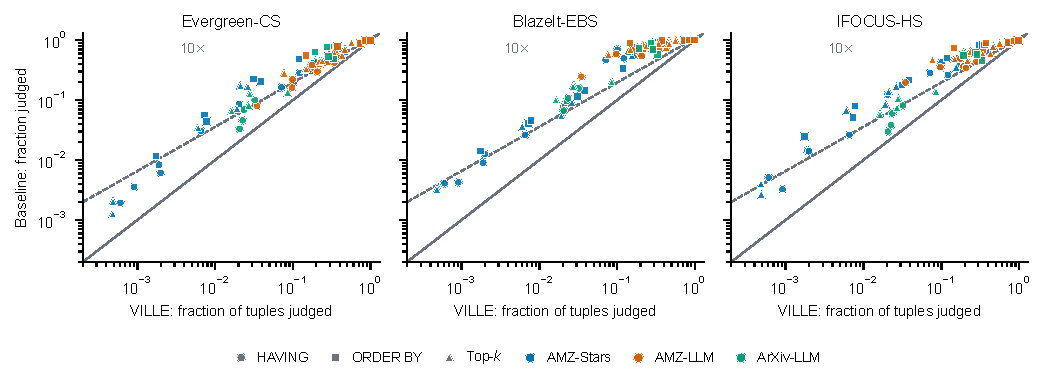
\includegraphics[width=\textwidth]{figures/fig_main_scatter.pdf}
\caption{Fraction of tuples judged per query: \sys{} (x-axis) against each certified baseline (y-axis). Each point is one query (mean over 30 executions); marker shape gives the query type and color the dataset. Points above the solid line cost the baseline more calls than \sys{}; points above the dashed line cost at least ten times more.}
\label{fig:main}
\end{figure*}

\sys{} judged at most as many tuples as Evergreen-CS and BlazeIt-EBS on every one of the \numNQ{} queries, and at most as many as IFOCUS-HS on all but one (\Cref{tab:main} and \Cref{fig:main}).
Across all queries, Evergreen-CS judged \numRWSR$\times$ as many tuples as \sys{} (geometric mean; up to \numRWSRMAX$\times$), BlazeIt-EBS \numRBSP$\times$, and IFOCUS-HS \numRHS$\times$.

The savings grow with group size: across all queries, the saving over Evergreen-CS rises with the mean group size (Spearman $\rho=\numRHOGS$), from \numBINA$\times$ for groups below 5{,}000 tuples to \numBINB$\times$ between 5{,}000 and 50{,}000 and \numBINC$\times$ above.
On ArXiv-LLM, which combines real LLM judgments with groups of 5{,}000 to 60{,}000 abstracts, Evergreen-CS judged \numAXRWSR$\times$ as many tuples as \sys{}, BlazeIt-EBS \numAXRBSP$\times$, and IFOCUS-HS \numAXRHS$\times$; finding the five years with the highest share of abstracts that claim to beat the state of the art took \sys{} 8{,}557 calls and Evergreen-CS 38{,}563.
On the category and year groupings of AMZ-Stars, whose groups hold $10^4$ to $10^6$ reviews, Evergreen-CS judged 4.4$\times$ and 5.2$\times$ as many tuples as \sys{}, and IFOCUS-HS 6.7$\times$ and 6.5$\times$.
For example, \sys{} answered the HAVING query on the share of negative reviews per year with 139{,}097 LLM calls, whereas Evergreen-CS, BlazeIt-EBS, and IFOCUS-HS needed 583{,}720, 434{,}123, and 847{,}783; ranking the 19 years by their share of five-star reviews took \sys{} 213{,}170 calls and Evergreen-CS 1.53 million.
On product groups, which hold one to thirty thousand reviews and often differ by little more than the margin, every certified method judges a large share of each group, and the finite-population form of the tests lets all of them stop once little uncertainty remains.
AMZ-LLM consists only of such groups (1{,}000 to 4{,}000 reviews per product, at most 16{,}704 per year).
There \sys{} judged \numAMZLRWSR$\times$ fewer tuples than Evergreen-CS, \numAMZLRBSP$\times$ fewer than BlazeIt-EBS, and \numAMZLRHS$\times$ fewer than IFOCUS-HS, with the largest gains on the year grouping (1.9$\times$ over Evergreen-CS).

Certification costs no more than common practice.
The usual procedure samples until normal-approximation intervals separate; it carries no guarantee, yet it judged \numRCLT$\times$ as many tuples as \sys{}.
Run on proxy-rectified values (CLT+P), the same procedure judged \numRCLTP$\times$ as many tuples, so \sys{} pays about \numRCLTPINV$\times$ the calls of this uncertified counterpart for a guarantee that holds at every stopping time.
Neither procedure is uncertified merely in principle: on AMZ-LLM, CLT returned an incorrect answer in up to 13\% of a query's executions and CLT+P in up to 7\%, while no certified method erred (\Cref{sec:validity}).
Skipping the LLM altogether is worse still: answering from each group's mean proxy score, which costs no LLM call, gave an answer that is not $r$-correct on \numNPROXYWRONG{} of the \numNPROXYQ{} queries.

\subsection{Live query execution}
\label{sec:live}

We measure how certification translates into query latency with two model families,
Qwen2.5-1.5B-Instruct and SmolLM2-1.7B-Instruct~\cite{smollm2}, on an RTX 4060 laptop GPU (8\,GB).
A DuckDB group-by supplies the product identifiers and row lists of the video-game reviews.
We select a shared workload of \numLiveN{} reviews in 16 products by uniformly sampling at most 2{,}000 evaluation reviews per product.
Selection uses metadata, and each model receives a separate proxy trained on its judgments of the existing disjoint 3{,}000-review training split.
Both models use the \textsc{Defect} prompt and the same query parameters, fixed before the additional judgments are collected.
The HAVING threshold is 0.20, the indifference margin is 0.01, $\alpha=0.05$, and $k=5$.

\begin{table*}[t]
\centering
\caption{Live execution with two model families over the same 32,000 reviews in 16 product groups: latency tracks the number of LLM calls, and certificate updates take at most \numLiveMaxOverhead\% of \sys{}'s latency.
CS denotes the Evergreen-style confidence-sequence baseline. Calls count fresh model evaluations by each method.
Latencies include prompt processing, model inference and certificate updates, with the model
resident and proxies prepared. Each model's complete exact scan is measured once and supplies the shared reference
latency for the three queries over the same predicate. The SQL aggregation time is added per query.
Speedup is measured exact-query latency divided by VILLE latency.}
\label{tab:online}
\footnotesize
\setlength{\tabcolsep}{5pt}
\renewcommand{\arraystretch}{1.12}
\begin{tabular}{llrrrrrr}
\toprule
& & \multicolumn{2}{c}{LLM calls} & \multicolumn{3}{c}{Measured latency (s)} & \\
\cmidrule(lr){3-4}\cmidrule(lr){5-7}
Model & Query & \sys{} & CS & \sys{} & CS & Exact & Speedup \\
\midrule
Qwen2.5-1.5B & HAVING & 12,400 & 15,100 & 229.3 & 280.0 & 570.3 & 2.49$\times$ \\
 & ORDER BY & 26,400 & 30,000 & 484.8 & 558.0 & 570.3 & 1.18$\times$ \\
 & Top-5 & 16,500 & 19,700 & 312.3 & 378.4 & 570.3 & 1.83$\times$ \\
\midrule
SmolLM2-1.7B & HAVING & 1,900 & 2,000 & 44.6 & 47.9 & 712.8 & 15.97$\times$ \\
 & ORDER BY & 32,000 & 31,500 & 709.2 & 699.6 & 712.8 & 1.00$\times$ \\
 & Top-5 & 23,700 & 25,400 & 515.5 & 556.1 & 712.7 & 1.38$\times$ \\
\bottomrule
\end{tabular}
\end{table*}


\sys{} and Evergreen-CS issue fresh model requests for every query, using the same random group permutations and 100-tuple request blocks.
The decision layer consumes the row lists, updates its certificates, and charges every tuple actually sent to the model.
The table reports one complete execution per configuration with the model resident and proxy scores prepared, following the amortized-proxy setting.
For each model, we also execute a complete scan of all \numLiveN{} reviews.
SQL aggregation of its judgments supplies the reference answers for HAVING, ORDER BY and Top-5.
The measured scan time is their shared exact-evaluation reference, with the SQL aggregation time added per query.

All six \sys{} answers are $r$-correct, and every live judgment agrees with the corresponding model's complete pass (\Cref{tab:online}).
Saved calls became saved time one for one: in all twelve sampled executions, the latency per call stayed within 8\% of that of the model's full scan, and certificate updates and query bookkeeping took at most \numLiveMaxOverhead\% of \sys{}'s latency.
The call counts of \Cref{sec:main} therefore translate directly into latency.
On Qwen2.5, HAVING takes 12{,}400 calls and 229.3\,s against 32{,}000 calls and 570.3\,s for full evaluation, a \numLiveHavingMin$\times$ speedup.
SmolLM2 reports a defect in under 10\% of every product's reviews, far below the threshold, so HAVING is certified after 1{,}900 calls and 44.6\,s against 712.8\,s, a \numLiveHavingMax$\times$ speedup.
With 2{,}000 reviews per product and a margin of one percentage point, ranking all 16 products requires most of each group; the workload isolates how calls convert into latency.

\subsection{Where the savings come from}
\label{sec:ablation}

\begin{figure}[t]
\centering
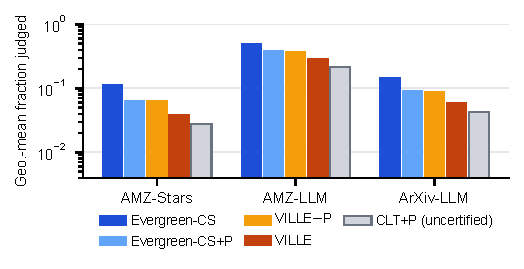
\includegraphics[width=\columnwidth]{figures/fig_decomposition.pdf}
\caption{Where the savings come from. Geometric-mean fraction of tuples judged over the queries of each dataset, for the Evergreen-style confidence sequence with and without the proxy, \sys{} with and without the proxy, and the uncertified CLT+P floor.}
\label{fig:decomp}
\end{figure}

\begin{figure}[t]
\centering
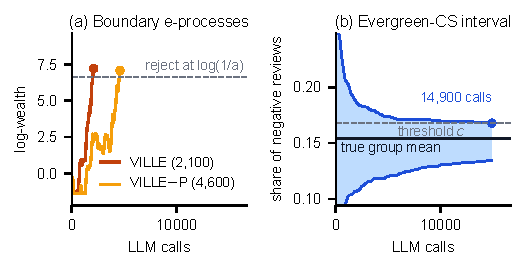
\includegraphics[width=\columnwidth]{figures/fig_anatomy.pdf}
\caption{One HAVING decision on AMZ-Stars: is the share of negative reviews in 2017 (752{,}784 reviews, true share 15.4\%) below the threshold of 16.8\%? (a) Log-wealth of the boundary test with and without the proxy, drawn until it reaches $\log(1/a)$. (b) The Evergreen-style confidence sequence, drawn until its upper bound falls below the threshold. One run; the same tuples are judged in the same order.}
\label{fig:anatomy}
\end{figure}

\Cref{fig:anatomy} dissects a single decision.
The 2017 group lies 1.6$r$ below the threshold.
The confidence sequence must shrink until its upper bound clears the threshold, which takes 14{,}900 calls.
The boundary test only has to accumulate evidence against one value and rejects after 4{,}600 calls without the proxy; betting on rectified values halves this again, to 2{,}100 calls.

Two mechanisms contribute about equally, and their effects multiply (\Cref{fig:decomp}).
Holding the confidence sequence fixed, adding the proxy (Evergreen-CS $\rightarrow$ Evergreen-CS+P) cut LLM calls by \numAMZSPROXYEFF$\times$ on AMZ-Stars, \numAMZLPROXYEFF$\times$ on AMZ-LLM, and \numAXPROXYEFF$\times$ on ArXiv-LLM (geometric means).
Holding the proxy fixed, the gap-adaptive boundary tests and direct paired construction (Evergreen-CS+P $\rightarrow$ \sys{}) cut them by a further \numAMZSBOUNDEFF$\times$, \numAMZLBOUNDEFF$\times$, and \numAXBOUNDEFF$\times$.
Without the proxy, \sys{}$-$P still judged \numAMZSBETVSWSR$\times$, \numAMZLBETVSWSR$\times$, and \numAXBETVSWSR$\times$ fewer tuples than Evergreen-CS, showing the contribution of these betting and paired-test choices.
For orderings, the paired tests add to this, because two confidence sequences must clear the gap together, whereas the paired test pays once for the deviation of the difference.
The proxy also repays its training labels: on the two LLM-judged datasets, \sys{} issued \numPROXYSAVEMIN{} to \numPROXYSAVEMAX{} thousand fewer calls per predicate than \sys{}$-$P over the queries we posed, against the 3{,}000 calls that trained each proxy.

\subsection{Proxy quality, margin, and scale}
\label{sec:sensitivity}

\begin{figure*}[t]
\centering
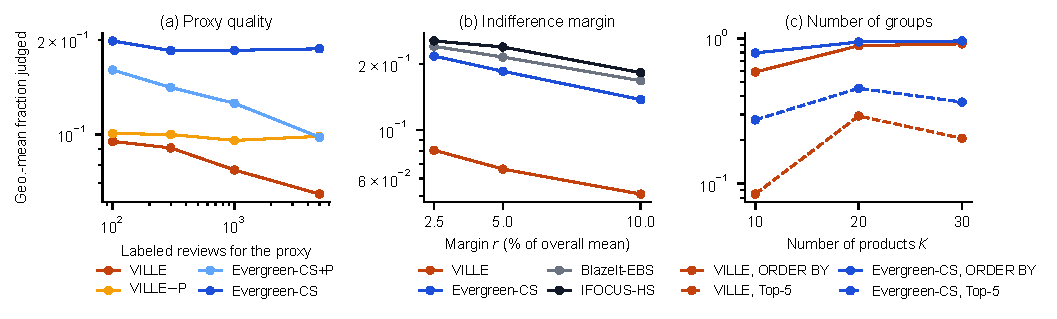
\includegraphics[width=\textwidth]{figures/fig_sensitivity.pdf}
\caption{Sensitivity on AMZ-Stars \textsc{Neg} queries (geometric mean over the year and Appliances-product groupings). (a) Proxies trained on 100 to 5{,}000 labeled reviews. (b) Indifference margin $r$. (c) Number of groups for ORDER BY and Top-5.}
\label{fig:sens}
\end{figure*}

Proxy quality governs the size of the saving, not its sign (\Cref{fig:sens}a).
We retrained the \textsc{Neg} proxy on 1{,}000, 300, and 100 of the 5{,}000 labeled reviews, which lowered its AUC from 0.960 to 0.941, 0.901, and 0.836.
With the weakest proxy, \sys{} judged 6\% fewer tuples than without a proxy; with the strongest, 35\% fewer.
In every case \sys{} stayed below Evergreen-CS, by 2.1$\times$ with the weakest proxy and 2.9$\times$ with the strongest, so even a proxy trained on 100 labels is worth using.

The margin trades precision for calls without changing the comparison (\Cref{fig:sens}b).
Halving $r$ from 5\% to 2.5\% of the overall mean raised \sys{}'s cost by 22\%, and doubling it to 10\% lowered the cost by 23\%; Evergreen-CS judged between 2.7$\times$ and 2.8$\times$ as many tuples at every margin.
The error level matters little, because the cost grows with $\log(1/\alpha)$ (\Cref{eq:cost}): tightening $\alpha$ from 0.05 to 0.01 raised \sys{}'s cost by 15\% and Evergreen-CS's by 13\%, and loosening it to 0.10 lowered both by 5\% to 6\%.

Cost depends on how close the groups are rather than on how many there are (\Cref{fig:sens}c).
Among the Appliances products, adding those ranked 11 to 20 by review count raised every method's cost, whereas adding products 21 to 30 lowered every method's Top-5 cost and changed each certified method's ORDER BY cost by at most 3\%, because the cost of a decision is driven by how close its groups are to each other.
\sys{} judged 1.4$\times$ to 1.9$\times$ fewer tuples than Evergreen-CS at 10, 20, and 30 groups (geometric mean over the three query forms), although the union bound over pairs grows quadratically with the number of groups.

\subsection{Validity}
\label{sec:validity}

\begin{table}[t]
\centering
\caption{Errors over all 75 queries, each executed 30 times. Answer errors violate the returned-result definition of $r$-correctness. Decision errors concern a group or pair used by the answer, at least $r$ from its boundary, certified on the wrong side or as indifferent. The last column is the highest per-query answer-error rate.}
\label{tab:validity}
\footnotesize
\begin{tabular}{lrrr}
\toprule
Method & Answers & Decisions & Worst rate \\
\midrule
\sys{} & 0 / 2250 & 0 / 2250 & 0.00 \\
\sys{}$-$P & 0 / 2250 & 0 / 2250 & 0.00 \\
Evergreen-CS & 0 / 2250 & 0 / 2250 & 0.00 \\
Evergreen-CS+P & 0 / 2250 & 0 / 2250 & 0.00 \\
BlazeIt-EBS & 0 / 2250 & 0 / 2250 & 0.00 \\
IFOCUS-HS & 0 / 2250 & 0 / 2250 & 0.00 \\
CLT (uncert.) & 5 / 2250 & 16 / 2250 & 0.13 \\
CLT+P (uncert.) & 3 / 2250 & 3 / 2250 & 0.07 \\
\bottomrule
\end{tabular}
\end{table}

No certified method returned an incorrect answer in any of the \numNEXEC{} query executions (\Cref{tab:validity}).
Uncertified CLT returned an incorrect answer in \numNCLTERR{} executions spread over \numNCLTERRQ{} queries, and CLT+P in \numNCLTPERR{} executions over \numNCLTPERRQ{} queries; the worst rates, 13\% and 7\%, occurred on AMZ-LLM queries about defects.
The normal approximation errs rarely, but silently: nothing in a single execution reveals when it has failed.
To probe the tests directly, we ran each test 2{,}000 times on finite populations whose mean sits exactly on the null boundary, a Bernoulli population of 20{,}000 tuples and a skewed population of 5{,}000 tuples, with $a=0.05$.
The one-sample tests rejected in 1.4\% to 2.1\% of runs and the paired test, applied to groups of 3{,}000 and 8{,}000 tuples, in 1.1\%, both below the nominal 5\%.

A misleading proxy costs calls but not correctness.
We replaced the \textsc{Neg} proxy on the year grouping by its inversion $1-p$, by uniform noise, and by a random permutation of its scores, and forced $\beta=1$ instead of letting cross-validation shrink it.
\sys{} remained error-free in all 90 executions.
Relative to \sys{}$-$P, its largest cost ratios were 1.71$\times$ with the inverted proxy, 1.55$\times$ with noise, and 1.16$\times$ with the permuted scores. It stayed below Evergreen-CS in every case.
The cross-validated coefficient used elsewhere downweights uninformative proxies toward $\beta=0$ and clips negatively correlated proxies to zero.

\subsection{Scope}
\label{sec:scope}

\sys{} assumes that the LLM judgment of a tuple is fixed once computed, which holds with deterministic decoding and caching, and that tuples are sampled uniformly within each group.
Its guarantee concerns the decisions that the LLM itself would reach on all tuples; the fidelity of the LLM to human judgment is a separate question that applies equally to exact evaluation.
The size of the saving depends on how well the proxy tracks the LLM in use, whereas the guarantee does not.
The union bound over groups and pairs is the simplest way to control all decisions at once.
Because every test produces an e-value, replacing the union bound by e-value-based false discovery rate control~\cite{wang2022ebh} is a direct extension for dashboards with hundreds of groups.

\section{Related Work}
\label{sec:related}

\paragraph*{LLM-powered query processing}
Semantic operators extend relational queries with natural-language filters, joins, rankings, and aggregations evaluated by LLMs~\cite{lotus,docetl,uqe,thalamusdb}.
Their optimizers reduce LLM calls with model cascades, proxies, and sampling.
LOTUS gives accuracy guarantees relative to a reference algorithm for filters, joins, and semantic group-by, and ranks tuples with LLM comparisons~\cite{lotus}.
BARGAIN certifies the precision, recall, or accuracy of cascaded LLM classifiers with betting-style tests~\cite{bargain}.
Evergreen verifies claims made in LLM-generated summaries of a relation by compiling each claim into a verification query; it estimates proportions with confidence sequences and stops early when a threshold claim is confirmed or refuted~\cite{evergreen}.
These systems certify tuple-level outputs or individual claims.
\sys{} targets group-level decision queries, tests their boundaries directly, and draws its savings from proxies that these confidence sequences do not use; we compare against an Evergreen-style confidence sequence in \Cref{sec:exp}.

\paragraph*{Proxy-assisted analytics over expensive predicates}
Video and unstructured-data analytics popularized cheap proxy models for expensive neural predicates~\cite{noscope,blazeit,supg,abae,tasti}.
BlazeIt uses proxy scores as control variates and stops with an empirical Bernstein bound~\cite{blazeit,mnih2008}; ABae stratifies on proxy scores and samples within strata for aggregation queries, including group-by keys~\cite{abae}; SUPG selects records under precision or recall targets~\cite{supg}; and BaS combines blocking and sampling to estimate analytical joins over unstructured data with statistical guarantees~\cite{bas}.
These methods estimate aggregates or select records, mostly with fixed-sample or central-limit guarantees.
\sys{} shares their premise that proxies should shape sampling, but uses the proxy inside an e-process so that the decision, not an estimate, is certified under continuous monitoring.

\paragraph*{Sampling-based decisions in visualization and AQP}
Online aggregation showed that users stop queries once running estimates look good enough~\cite{ola}.
IFOCUS orders bar-chart groups with Hoeffding--Serfling intervals and a union bound over rounds~\cite{ifocus}; SeeDB prunes candidate views with confidence intervals~\cite{seedb}; Macke et~al.\ tighten distribution-sensitive intervals and note that intervals can stop HAVING queries early~\cite{macke2021}.
PilotDB provides a priori error guarantees for approximate queries with block sampling~\cite{pilotdb}.
These works decide on cheap-to-read data and rely on range-based or fixed-sample bounds; \sys{} targets the regime in which every sample is an LLM call and tightens decisions with variance-adaptive betting and proxies.

\paragraph*{Anytime-valid inference}
Ville's inequality~\cite{ville1939} underlies confidence sequences~\cite{darling1967,howard2021} and the e-value framework for safe, anytime-valid inference~\cite{shafer2021,ramdas2023savi,grunwald2024}.
Betting-based confidence sequences give tight, variance-adaptive intervals for bounded means, including sampling without replacement~\cite{wsr2024betting,wsr2020wor}.
Prediction-powered inference combines model predictions with a few labels~\cite{ppi}, and recent work extends it to anytime-valid confidence sequences~\cite{avppi} and to e-values~\cite{ppevalues}.
\sys{} applies the same rectifier to a finite population, in which every group's proxy mean is known exactly and tuples are drawn without replacement, and it tests only the boundaries that decide a query, for many groups at once.
Best-arm and top-$k$ identification with indifference zones goes back to sequential selection~\cite{bechhofer1954} and LUCB-style algorithms~\cite{lucb}.
\sys{} builds on these tools; its contribution is a query-processing layer that compiles HAVING, ORDER BY, and Top-$k$ queries into boundary e-processes, rectifies them with proxies under finite-population sampling, and pairs groups of very different sizes.

\section{Conclusion}
\label{sec:conclusion}

Decision queries over LLM-evaluated attributes ask for discrete answers, and discrete answers can be certified far more cheaply than precise estimates.
\sys{} compiles HAVING, ORDER BY, and Top-$k$ queries into boundary hypotheses, tests each with a betting e-process on proxy-rectified values, and stops each group as soon as its decisions are certified.
The answer is $r$-correct with probability at least $1-\alpha$ under any stopping rule and any proxy.
On \numNQ{} queries over 6.8 million reviews and over 431 thousand reviews and paper abstracts judged by a real LLM, \sys{} returned no incorrect answer and needed \numRWSR$\times$ fewer LLM calls than Evergreen-style confidence sequences and \numRHS--\numRBSP$\times$ fewer than IFOCUS- and BlazeIt-style bounds, about as many as uncertified sampling.
The savings are largest where they matter most, on large groups, where \sys{} judged up to \numRWSRMAX$\times$ fewer tuples than an Evergreen-style confidence sequence.
With Qwen2.5 and SmolLM2 in the loop, latency followed the number of calls, and HAVING queries ran \numLiveHavingMin$\times$ and \numLiveHavingMax$\times$ faster than full evaluation.
The same construction applies wherever a per-tuple evaluation is expensive and a cheap correlate exists, such as vision models over images or human labels over records.


\section*{AI-Generated Content Acknowledgment}
Claude (Anthropic) assisted drafting and editing throughout the manuscript and development of experiment, figure, and table code. OpenAI Codex assisted development and validation of the cached and live query execution, result aggregation, and manuscript revisions, including \Cref{sec:processing,sec:exp}, and construction of the vector artwork and drawing script of \Cref{fig:overview}. These tools also assisted literature search and reference checking. The authors take responsibility for the correctness and originality of the submitted work.

\IEEEtriggeratref{17}
\bibliographystyle{IEEEtran}
\bibliography{refs}
\end{document}
